
% This LaTeX was auto-generated from an M-file by MATLAB.
% To make changes, update the M-file and republish this document.

\documentclass[12pt]{article}

%% Pacotes matlab
\usepackage{graphicx}
\usepackage{color}

%% Escrevendo em portugu�s:
\usepackage[brazil]{babel}
\usepackage[latin1]{inputenc} 
\usepackage[T1]{fontenc}
\usepackage{epsfig}
\usepackage{psfrag}
\usepackage{fullpage}
\usepackage{setspace}
%----------------------------


\newtheorem{teorema}{Teorema}%[chapter]
\newtheorem{problema}[teorema]{Problema}
\newtheorem{conj}[teorema]{Conjectura}
\newtheorem{lema}[teorema]{Lema}
\newtheorem{exerc}[teorema]{Exercício}


% Ad hoc macros
\newcommand{\qed}       {\hfill\Box}
\newcommand{\card}[1]   {\left|#1\right|}
\newcommand{\nct}       {\chi_{_T}}
\newcommand{\cnk}[2]    {C_{#1}^{#2}}
\newcommand{\ed}[2]     {#1#2}
\newcommand{\teto}[1]   {\lceil #1 \rceil}
\newcommand{\piso}[1]   {\lfloor #1 \rfloor}
\newcommand{\itab}[1]{\hspace{0em}\rlap{#1}}
\newcommand{\tab}[1]{\hspace{.2\textwidth}\rlap{#1}}


\begin{document}

    
    
\subsection*{Contents}

\begin{itemize}
\setlength{\itemsep}{-1ex}
   \item ES868 � Pr� Relat�rio Lab 3
   \item Controlador proporcional
   \item Controlador de Ziegler Nichols
\end{itemize}


\subsection*{ES868 � Pr� Relat�rio Lab 3}

\begin{par}
\textbf{Controle de plantas eletr�onicas utilizando um controlador PID digital}
\end{par} \vspace{1em}
\begin{par}
Turma A - 16/03/2015
\end{par} \vspace{1em}
\begin{itemize}
\setlength{\itemsep}{-1ex}
   \item Augusto Miranda Garcia - 104627
   \item Guilherme de Oliveira Souza � 117093
   \item Vin�cius Ragazi David - 120258
\end{itemize}
\begin{verbatim}
load ../G.mat
s = tf('s');
\end{verbatim}


\subsection*{Controlador proporcional}

\begin{par}
Para se obter o tempo m�nimo de estabiliza��o, os p�los de malha fechadas tem de estar � mais esquerda poss�vel. Observando o root locus da planta:
\end{par} \vspace{1em}
\begin{verbatim}
rlocus(G)
\end{verbatim}

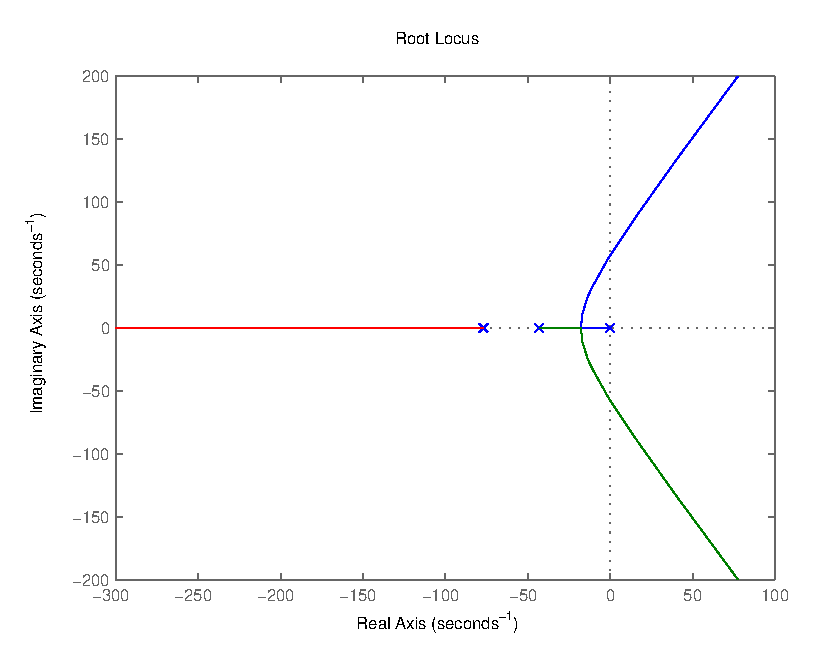
\includegraphics [width=4in]{pre_relatorio_01.eps}
\begin{par}
Pode-se observar que isso ir� ocorrer quando os dois p�los (verde e azul na figura) se encontrarem, no ponto pr�ximo de -20. Para obter a coordenada exata desse ponto, pode-se verificar a multiplicidade das ra�zes da equa��o carater�stica $1 + k G(s) = 0$.
\end{par} \vspace{1em}
\begin{par}
No nosso caso, com $G(s) = \frac{P(s)}{Q(s)} = \frac{A}{B s^3 + C s^2 + D s + E}$ , $k(s) = -\frac{B s^3 + C s^2 + D s + E}{A}$.
\end{par} \vspace{1em}
\begin{par}
Como o ponto buscando � raiz dupla de $k(s)$, ele � raiz da derivada de $k(s)$ em $s$, ou seja, raiz de $-\frac{3 B s^2 + 2 C s + D}{A}$.
\end{par} \vspace{1em}
\begin{par}
Substituindo os valores dos coeficientes e resolvendo, chegamos em
\end{par} \vspace{1em}
\begin{verbatim}
A = G.num{1}(4);
den = G.den{1};
raizes = roots(-polyder(den)/A)
\end{verbatim}

        \color{lightgray} \begin{verbatim}
raizes =

  -62.2543
  -17.7369

\end{verbatim} \color{black}
    \begin{par}
Observando o gr�fico do root locus mostrado anteriormente, sabemos ent�o que o valor buscado � $s = -17.7369$ e
\end{par} \vspace{1em}
\begin{verbatim}
k = -polyval(den, -17.7369)/A
\end{verbatim}

        \color{lightgray} \begin{verbatim}
k =

    0.8925

\end{verbatim} \color{black}
    \begin{par}
A resposta � rampa do controlador � exibida abaixo:
\end{par} \vspace{1em}
\begin{verbatim}
dt = 0.001;
t = 0:dt:5;
rampa = t;
sistema = feedback(k*G, 1);
lsim(sistema, rampa, t);
title('Resposta � rampa do controlador proporcional');
\end{verbatim}

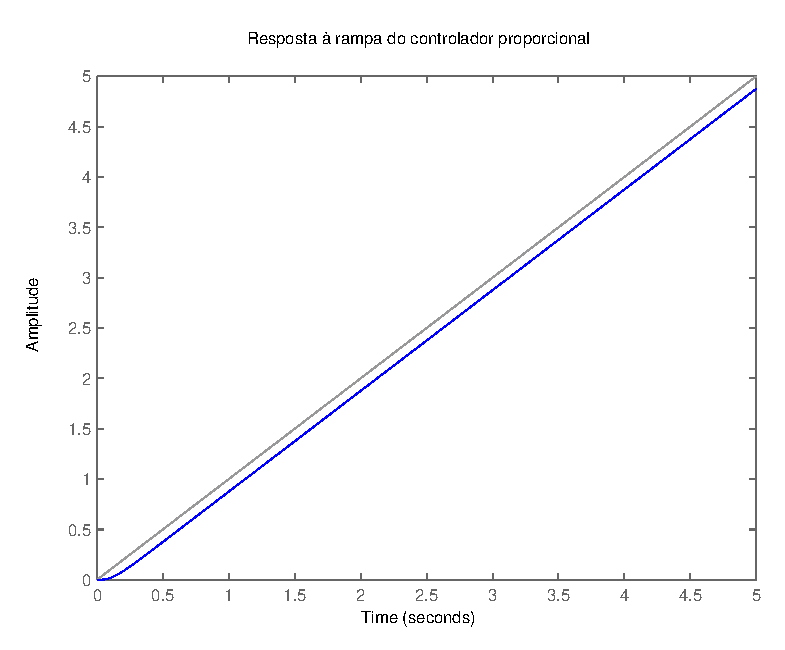
\includegraphics [width=4in]{pre_relatorio_02.eps}
\begin{par}
Entrada quadrada de amplitude 1 e 0.25Hz
\end{par} \vspace{1em}
\begin{verbatim}
onda_quadrada = square(2*pi*0.25*t)*0.5+0.5;
plot(t, onda_quadrada);
ylim([-0.1, 1.1]);
title('Entrada quadrada');
xlabel('t (s)');
\end{verbatim}

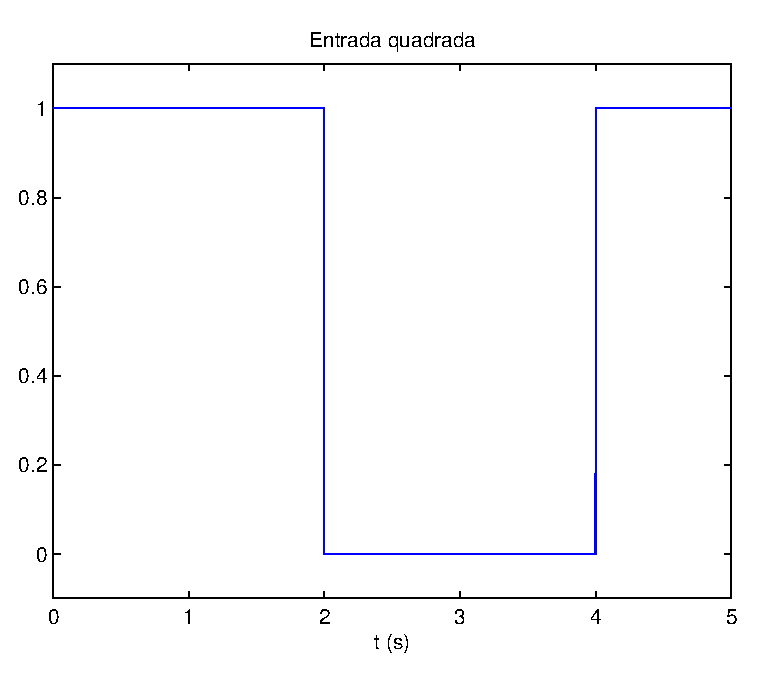
\includegraphics [width=4in]{pre_relatorio_03.eps}
\begin{par}
Resposta � onda quadrada
\end{par} \vspace{1em}
\begin{verbatim}
lsim(sistema, k*(1-sistema), 'g:', onda_quadrada, t);
title('Reposta � onda quadrada');
legend('y(t)', 'u(t)');
\end{verbatim}

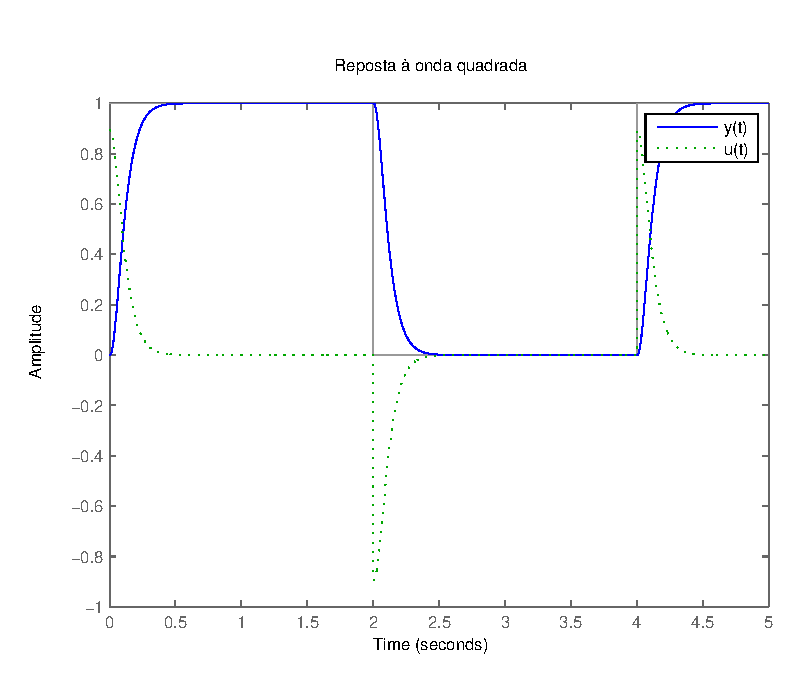
\includegraphics [width=4in]{pre_relatorio_04.eps}
\begin{par}
Entrada de rampa
\end{par} \vspace{1em}
\begin{verbatim}
onda_rampa = cumsum(onda_quadrada)*dt;
plot(t, onda_rampa);
title('Entrada em rampa');
xlabel('t (s)');
\end{verbatim}

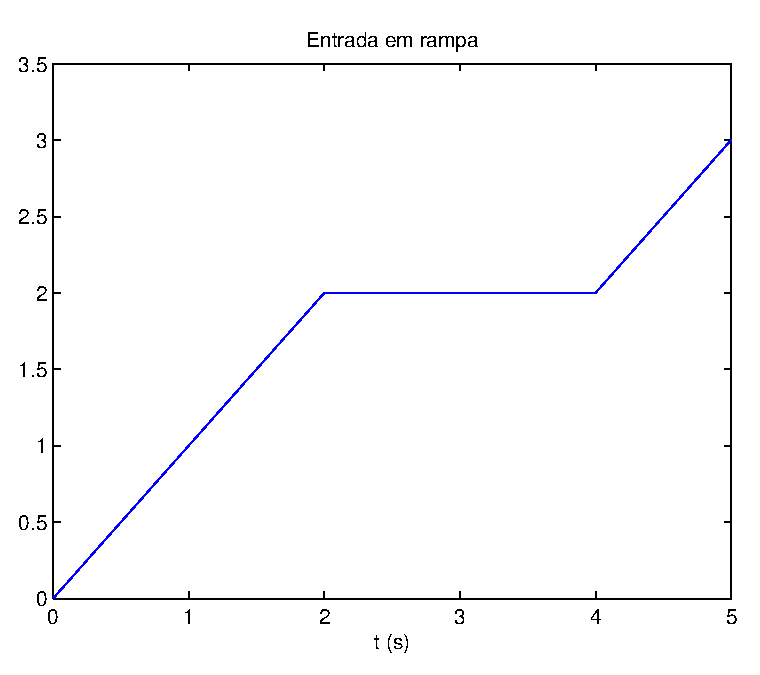
\includegraphics [width=4in]{pre_relatorio_05.eps}
\begin{par}
Resposta � rampa
\end{par} \vspace{1em}
\begin{verbatim}
lsim(sistema, k*(1-sistema), '-.', onda_rampa, t);
title('Reposta � rampa');
legend('y(t)', 'u(t)');
\end{verbatim}

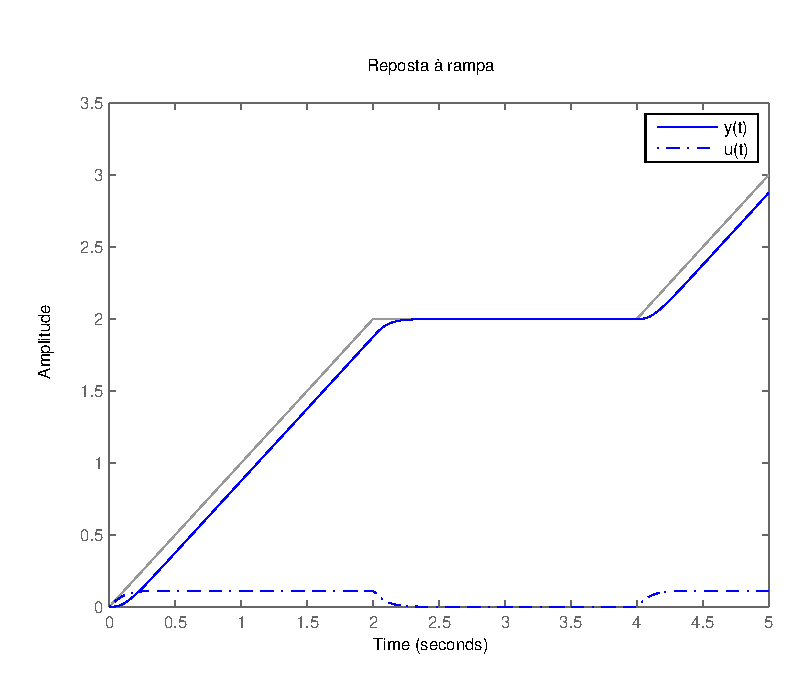
\includegraphics [width=4in]{pre_relatorio_06.eps}


\subsection*{Controlador de Ziegler Nichols}

\begin{par}
O primeiro passo no m�todo de Ziegler Nichols � encontrar $k = k_{osc}$ que deixa a planta no limiar de estabilidade quando em malha fechada:
\end{par} \vspace{1em}
\begin{par}
Para isso pode ser usado o crit�rio de Routh com a equa��o caracter�stica:
\end{par} \vspace{1em}
\begin{par}
$$1 + k G(s) = 0$$
\end{par} \vspace{1em}
\begin{par}
$$1 + \frac{8.993 k}{0.0003019 s^3 + 0.03622 s^2 + s} = 0$$
\end{par} \vspace{1em}
\begin{par}
$$\frac{0.0003019 s^3 + 0.03622 s^2 + s + 8.993 k}{0.0003019 s^3 + 0.03622 s^2 + s} = 0$$
\end{par} \vspace{1em}
\begin{par}
$$0.0003019 s^3 + 0.03622 s^2 + s + 8.993 k = 0$$
\end{par} \vspace{1em}
\begin{par}
Com o crit�rio de Routh chega-se em: $k = \frac{0.03622}{0.0003019 * 8.993} = 13.3408$
\end{par} \vspace{1em}
\begin{verbatim}
k_osc = 13.3408;
GC_mf = feedback(G*k_osc,1);
poles = esort(pole(GC_mf));
w_osc = abs(poles(1));
T_osc = 2*pi/w_osc;
kp = 0.6*k_osc;
Ti = T_osc/2;
Td = T_osc/8;
C = kp*(1 + 1/(Ti*s) + Td*s)
\end{verbatim}

        \color{lightgray} \begin{verbatim}
C =
 
  0.005963 s^2 + 0.4369 s + 8.004
  -------------------------------
             0.05459 s
 
Continuous-time transfer function.

\end{verbatim} \color{black}
    \begin{par}
Usando o sisotool para ajustar o valor de kp e melhorar o desempenho do controlador, obtemos $kp_2 = 1.31 kp$.
\end{par} \vspace{1em}
\begin{par}
Compara��o antes vs depois da altera��o manual do lugar dos p�los:
\end{par} \vspace{1em}
\begin{par}

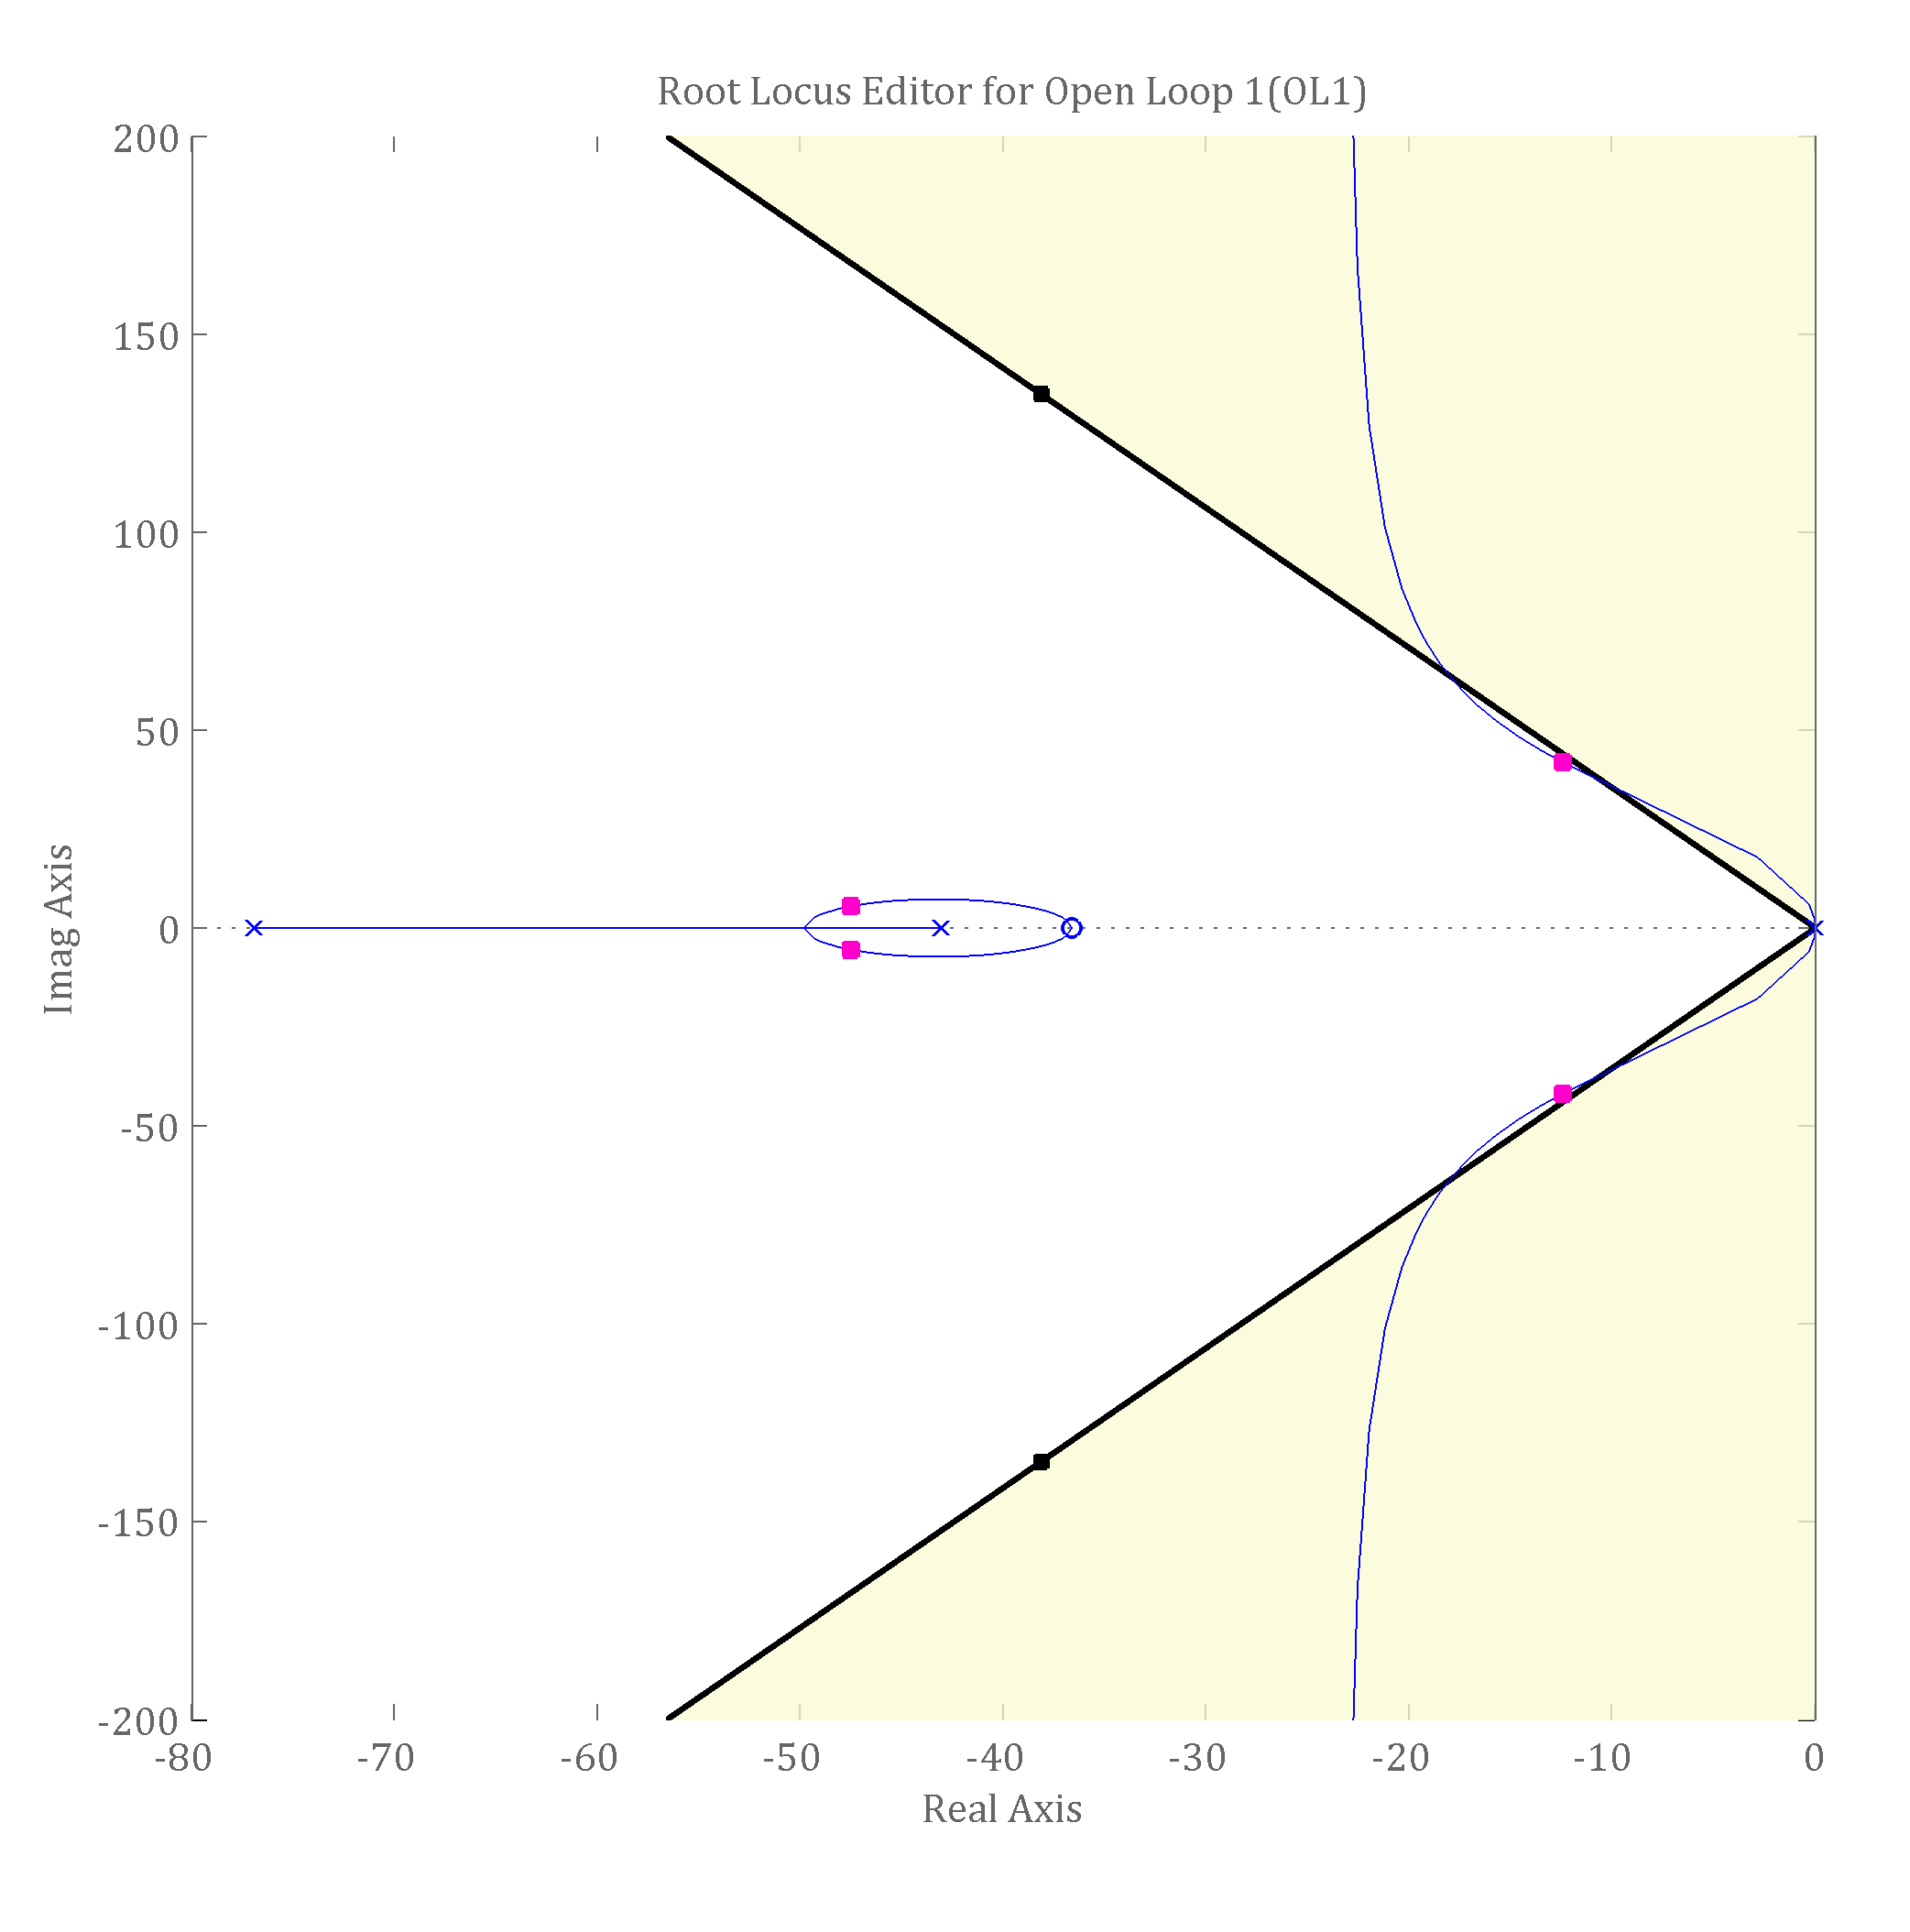
\includegraphics [width=4in]{../imgs/ziegler-nichols.png}

\end{par} \vspace{1em}
\begin{verbatim}
kp_2 = 1.31*kp;
C_2 = 1.31*C
\end{verbatim}

        \color{lightgray} \begin{verbatim}
C_2 =
 
  0.007811 s^2 + 0.5724 s + 10.49
  -------------------------------
             0.05459 s
 
Continuous-time transfer function.

\end{verbatim} \color{black}
    \begin{par}
C�lculo dos valores de desempenho
\end{par} \vspace{1em}
\begin{verbatim}
sistema = feedback(G*C_2, 1);
\end{verbatim}
\begin{par}

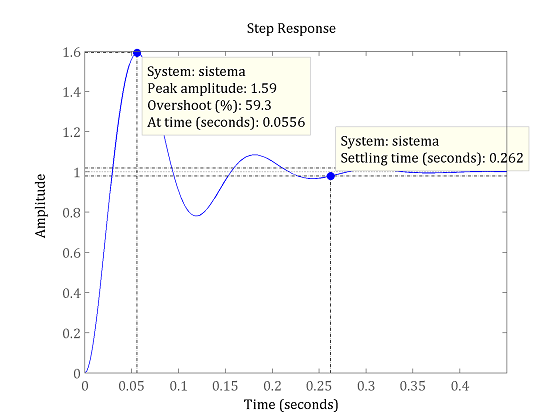
\includegraphics [width=4in]{../imgs/ziegler-nichols_step.png}

\end{par} \vspace{1em}
\begin{par}
Desempenho do sistema discreto
\end{par} \vspace{1em}
\begin{verbatim}
Ts = 0.001;
Gz = c2d(G, Ts, 'zoh');
Cz = c2d(C_2, Ts, 'matched');
sistemaZ = feedback(Gz*Cz, 1);
\end{verbatim}
\begin{par}

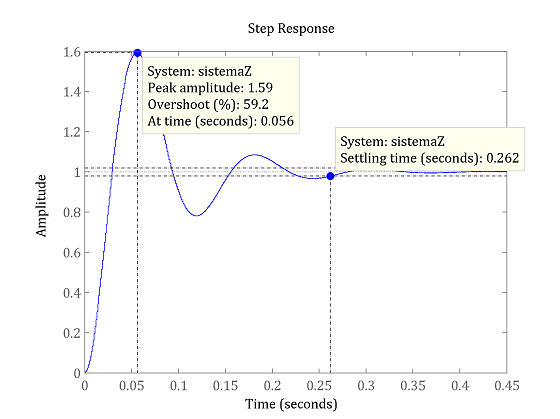
\includegraphics [width=4in]{../imgs/ziegler-nichols_z_step.png}

\end{par} \vspace{1em}
\begin{par}
Simula��o do sistema discreto
\end{par} \vspace{1em}
\begin{verbatim}
lsim(sistemaZ, onda_quadrada, t), snapnow;
lsim(sistemaZ, onda_rampa, t)
\end{verbatim}

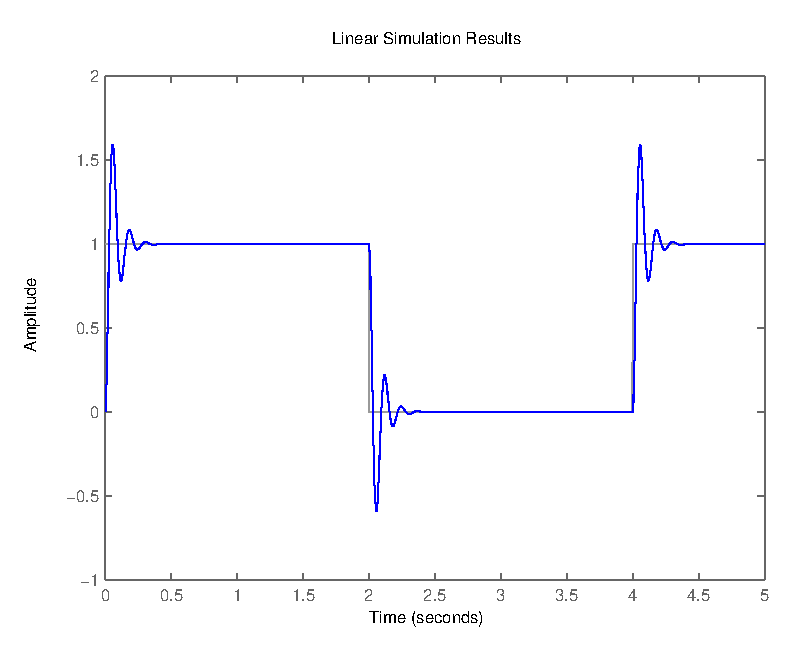
\includegraphics [width=4in]{pre_relatorio_07.eps}

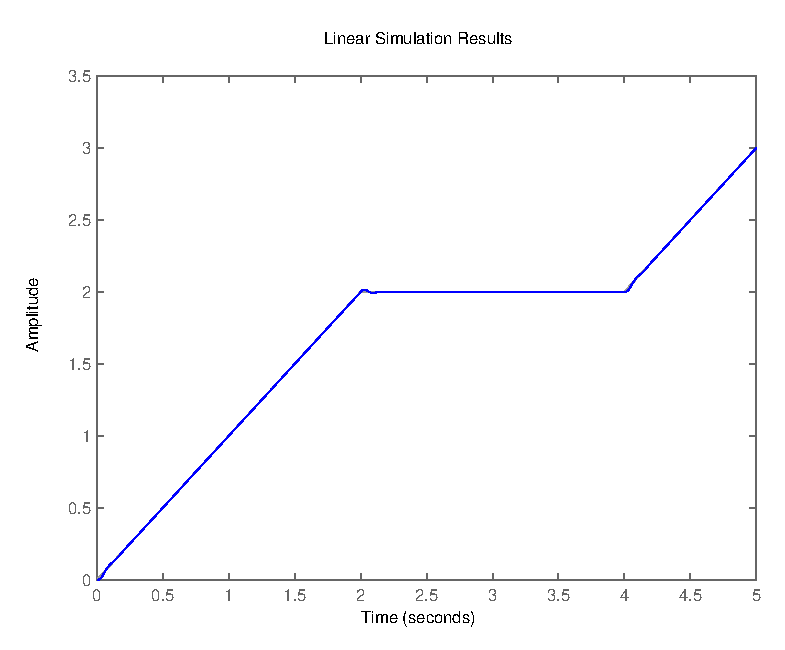
\includegraphics [width=4in]{pre_relatorio_08.eps}



\end{document}
    
